\documentclass[11pt,a4paper]{article}
\usepackage[utf8]{inputenc}
\usepackage[margin=2cm]{geometry}
\usepackage{tikz}
\usetikzlibrary{arrows.meta,positioning,calc,fit,backgrounds,decorations.pathreplacing,shapes.geometric}
\usepackage{xcolor}
\usepackage{enumitem}
\usepackage{amsmath,amssymb}
\usepackage{booktabs}
\usepackage{hyperref}
\usepackage{float}
\usepackage{tabularx}

\definecolor{teachcol}{RGB}{41,128,185}
\definecolor{studcol}{RGB}{39,174,96}
\definecolor{clustcol}{RGB}{142,68,173}
\definecolor{structcol}{RGB}{211,84,0}
\definecolor{physcol}{RGB}{231,76,60}
\definecolor{datacol}{RGB}{52,152,219}
\definecolor{greycol}{RGB}{127,140,141}
\definecolor{darkcol}{RGB}{44,62,80}
\definecolor{lightbg}{RGB}{246,248,250}

\title{\textbf{The $\Psi$-NN Paper Explained as an Architecture Pipeline}\\[0.2cm]
\large A brief and graphical explanation of how $\Psi$-NN automatically discovers structure\\[0.1cm]
\normalsize Liu et al.\ (2025), Nature Communications}
\author{}
\date{}

\begin{document}
\maketitle

\section{What Is the Main Idea?}

The paper solves one simple problem:

\begin{center}
\fbox{\parbox{0.86\textwidth}{
\centering
A standard PINN can solve the physics, but its internal connections are messy.\\[3pt]
$\Psi$-NN learns the physics first, then \textbf{discovers which connections are truly necessary}, and finally rebuilds a \textbf{smaller structured network}.
}}
\end{center}

So the paper is not mainly about inventing a new PDE solver. It is about \textbf{turning a trained physics network into an interpretable architecture}.

\section{Complete Pipeline as an Architecture}

\begin{center}
\resizebox{\textwidth}{!}{%
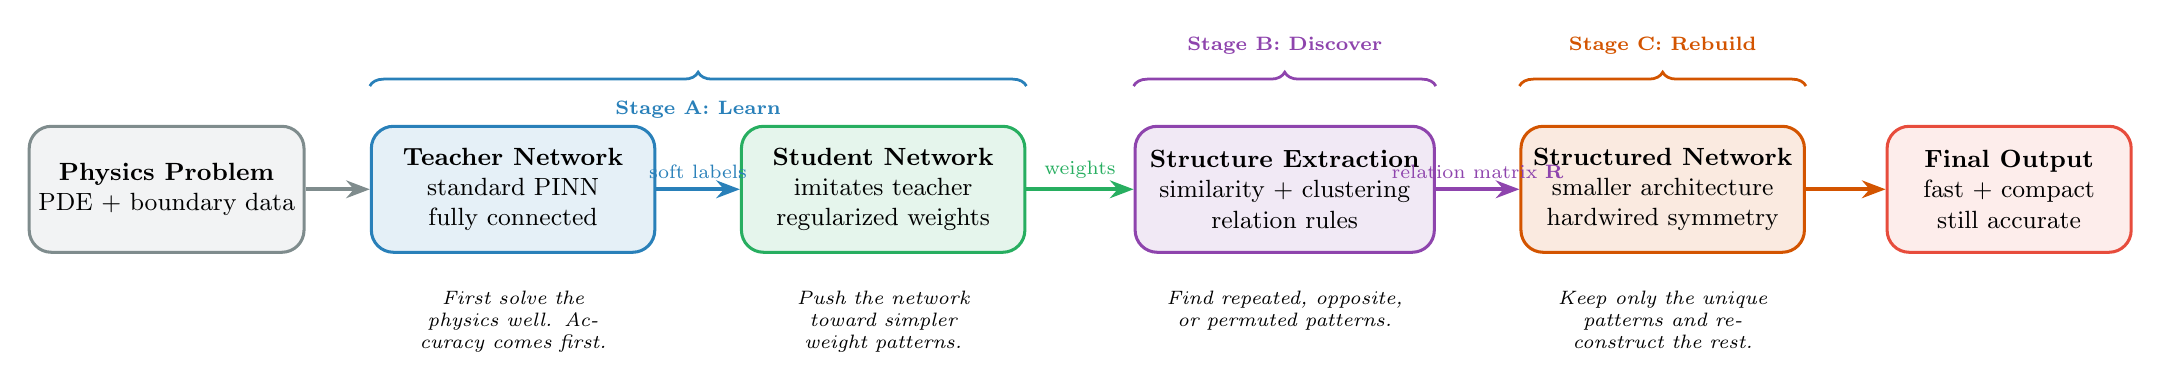
\begin{tikzpicture}[
    >={Stealth[length=3mm]},
    block/.style={rectangle, rounded corners=8pt, minimum height=1.6cm, align=center, font=\small, draw, line width=1.1pt},
    note/.style={font=\scriptsize\itshape, text width=3.1cm, align=center},
    arrow/.style={->, thick, line width=1.3pt},
]

\node[block, minimum width=3.1cm, fill=greycol!10, draw=greycol] (inp) at (0,0) {\textbf{Physics Problem}\\PDE + boundary data};
\node[block, minimum width=3.6cm, fill=teachcol!12, draw=teachcol] (teacher) at (4.4,0) {\textbf{Teacher Network}\\standard PINN\\fully connected};
\node[block, minimum width=3.6cm, fill=studcol!12, draw=studcol] (student) at (9.1,0) {\textbf{Student Network}\\imitates teacher\\regularized weights};
\node[block, minimum width=3.8cm, fill=clustcol!12, draw=clustcol] (extract) at (14.2,0) {\textbf{Structure Extraction}\\similarity + clustering\\relation rules};
\node[block, minimum width=3.6cm, fill=structcol!12, draw=structcol] (rebuild) at (19.0,0) {\textbf{Structured Network}\\smaller architecture\\hardwired symmetry};
\node[block, minimum width=3.1cm, fill=physcol!10, draw=physcol] (out) at (23.4,0) {\textbf{Final Output}\\fast + compact\\still accurate};

\draw[arrow, greycol] (inp) -- (teacher);
\draw[arrow, teachcol] (teacher) -- node[above, font=\scriptsize] {soft labels} (student);
\draw[arrow, studcol] (student) -- node[above, font=\scriptsize] {weights} (extract);
\draw[arrow, clustcol] (extract) -- node[above, font=\scriptsize] {relation matrix $\mathbf{R}$} (rebuild);
\draw[arrow, structcol] (rebuild) -- (out);

\node[note, below=10pt of teacher] {First solve the physics well. Accuracy comes first.};
\node[note, below=10pt of student] {Push the network toward simpler weight patterns.};
\node[note, below=10pt of extract] {Find repeated, opposite, or permuted patterns.};
\node[note, below=10pt of rebuild] {Keep only the unique patterns and reconstruct the rest.};

\draw[decorate, decoration={brace, amplitude=5pt, raise=14pt}, teachcol, line width=1pt] (teacher.north west) -- (student.north east);
\node[font=\scriptsize\bfseries, text=teachcol, above=22pt of $(teacher)!0.5!(student)$] {Stage A: Learn};

\draw[decorate, decoration={brace, amplitude=5pt, raise=14pt}, clustcol, line width=1pt] (extract.north west) -- (extract.north east);
\node[font=\scriptsize\bfseries, text=clustcol, above=22pt of extract] {Stage B: Discover};

\draw[decorate, decoration={brace, amplitude=5pt, raise=14pt}, structcol, line width=1pt] (rebuild.north west) -- (rebuild.north east);
\node[font=\scriptsize\bfseries, text=structcol, above=22pt of rebuild] {Stage C: Rebuild};
\end{tikzpicture}
}%
\end{center}

\section{Stage A: Learn the Physics First}

The paper separates two jobs that normally interfere with each other:

\begin{center}
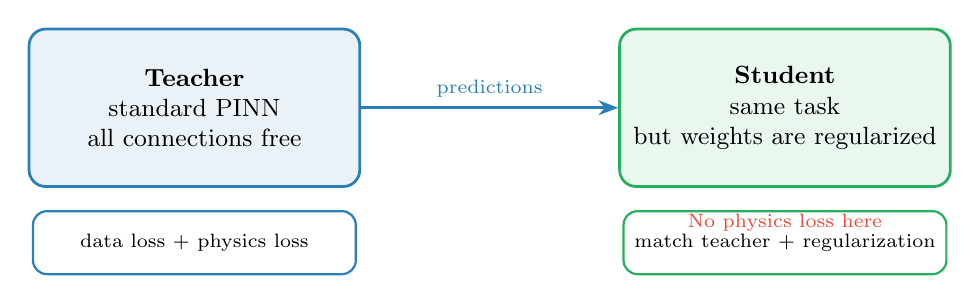
\begin{tikzpicture}[
    >={Stealth[length=2.5mm]},
    box/.style={rectangle, rounded corners=6pt, minimum width=4.2cm, minimum height=2cm, align=center, font=\small, draw, line width=1pt},
    loss/.style={rectangle, rounded corners=5pt, minimum width=4.1cm, minimum height=0.8cm, align=center, font=\scriptsize, draw, line width=0.8pt, fill=white},
]
\node[box, fill=teachcol!10, draw=teachcol] (t) at (0,0) {\textbf{Teacher}\\standard PINN\\all connections free};
\node[loss, below=8pt of t, draw=teachcol] {data loss + physics loss};

\node[box, fill=studcol!10, draw=studcol] (s) at (7.5,0) {\textbf{Student}\\same task\\but weights are regularized};
\node[loss, below=8pt of s, draw=studcol] {match teacher + regularization};

\draw[->, thick, teachcol, line width=1.2pt] (t) -- node[above, font=\scriptsize] {predictions} (s);
\node[font=\scriptsize, text=physcol, below=6pt of s.south] {No physics loss here};
\end{tikzpicture}
\end{center}

\textbf{Why two networks?} Because if one network tries to satisfy physics and become sparse at the same time, the optimization conflicts. The teacher learns the correct answer first. The student then learns a cleaner version of the same answer.

\section{Stage B: How Does $\Psi$-NN Discover the Best Structure Automatically?}

This is the key part.

The paper starts from the \textbf{trained student weights}. Then it asks:

\begin{center}
\fbox{\parbox{0.84\textwidth}{
\centering
Which neurons and connections are really different, and which ones are only repeated versions of the same physical pattern?
}}
\end{center}

\subsection*{Architecture View of the Discovery Step}

\begin{center}
\begin{tikzpicture}[
    >={Stealth[length=2.3mm]},
    step/.style={rectangle, rounded corners=6pt, minimum width=3.1cm, minimum height=1.5cm, align=center, font=\scriptsize, draw, line width=0.95pt},
    arrow/.style={->, thick, line width=1.1pt},
]
\node[step, fill=studcol!10, draw=studcol] (a) at (0,0) {\textbf{1. Read student weights}\\all layer matrices};
\node[step, fill=clustcol!10, draw=clustcol] (b) at (4,0) {\textbf{2. Measure similarity}\\same? opposite?\\permuted?};
\node[step, fill=clustcol!10, draw=clustcol] (c) at (8,0) {\textbf{3. Cluster weights}\\group similar rows\\or neurons};
\node[step, fill=structcol!10, draw=structcol] (d) at (12,0) {\textbf{4. Build rules}\\reuse, sign flip,\\swap, remove};
\node[step, fill=physcol!10, draw=physcol] (e) at (16,0) {\textbf{5. Keep prototypes}\\only unique patterns};

\draw[arrow, studcol] (a) -- (b);
\draw[arrow, clustcol] (b) -- (c);
\draw[arrow, clustcol] (c) -- (d);
\draw[arrow, structcol] (d) -- (e);
\end{tikzpicture}
\end{center}

In plain language, the discovery is done in five detailed steps:

\begin{enumerate}[leftmargin=*]
    \item \textbf{Read the trained student matrices.} Each layer contains many rows of weights. Each row corresponds to one neuron or one learned feature.
    \item \textbf{Compare rows with each other.} If two rows are almost identical, they probably represent the same physical behavior. If one row is approximately the negative of another, that suggests anti-symmetry. If the entries are the same but reordered, that suggests permutation symmetry.
    \item \textbf{Cluster similar rows.} The paper uses clustering to group weight rows that behave almost the same. This reveals how many \textit{truly unique} patterns exist.
    \item \textbf{Convert patterns into rules.} Instead of storing every row independently, the paper writes rules such as: row 4 = row 1, row 6 = $-$row 2, row 8 = swap(row 3), bias 5 = 0.
    \item \textbf{Choose the best structure.} ``Best'' means: the \textbf{simplest structure that still reproduces the teacher accurately}. So the method removes as much redundancy as possible without damaging the solution.
\end{enumerate}

\subsection*{What Does It Look For Inside the Network?}

\begin{center}
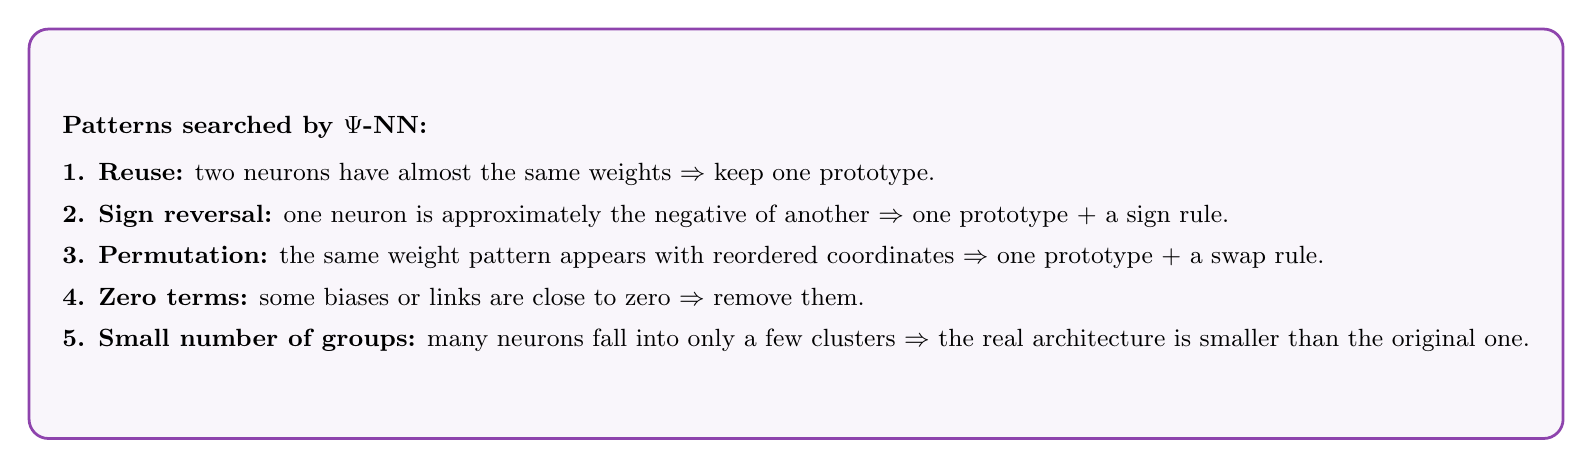
\begin{tikzpicture}[font=\small]
\node[rectangle, rounded corners=7pt, minimum width=13cm, minimum height=5.2cm, align=left,
      draw=clustcol, line width=1pt, fill=clustcol!5, inner sep=12pt] {
\textbf{Patterns searched by $\Psi$-NN:}\\[6pt]
\textbf{1. Reuse:} two neurons have almost the same weights $\Rightarrow$ keep one prototype.\\[4pt]
\textbf{2. Sign reversal:} one neuron is approximately the negative of another $\Rightarrow$ one prototype + a sign rule.\\[4pt]
\textbf{3. Permutation:} the same weight pattern appears with reordered coordinates $\Rightarrow$ one prototype + a swap rule.\\[4pt]
\textbf{4. Zero terms:} some biases or links are close to zero $\Rightarrow$ remove them.\\[4pt]
\textbf{5. Small number of groups:} many neurons fall into only a few clusters $\Rightarrow$ the real architecture is smaller than the original one.
};
\end{tikzpicture}
\end{center}

\subsection*{A Small Visual Example}

\begin{center}
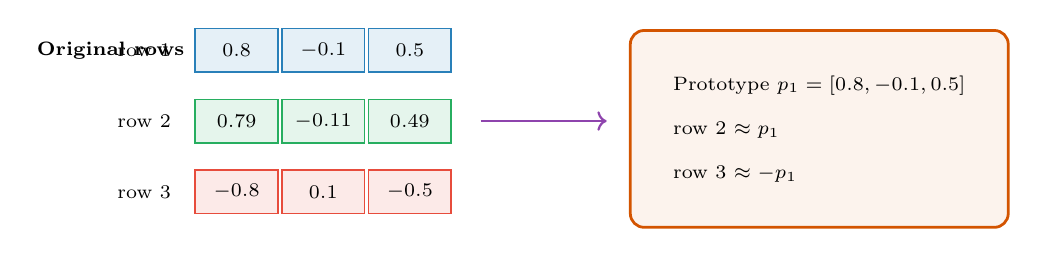
\begin{tikzpicture}[
    cell/.style={rectangle, minimum width=1.05cm, minimum height=0.55cm, draw, line width=0.6pt, font=\scriptsize, align=center},
    lab/.style={font=\scriptsize\bfseries},
]
\node[lab] at (-0.6,2.2) {Original rows};
\node[cell, fill=teachcol!12, draw=teachcol] (r1a) at (1,2.2) {$0.8$};
\node[cell, fill=teachcol!12, draw=teachcol] (r1b) at (2.1,2.2) {$-0.1$};
\node[cell, fill=teachcol!12, draw=teachcol] (r1c) at (3.2,2.2) {$0.5$};
\node[font=\scriptsize, left=5pt of r1a] {row 1};

\node[cell, fill=studcol!12, draw=studcol] (r2a) at (1,1.3) {$0.79$};
\node[cell, fill=studcol!12, draw=studcol] (r2b) at (2.1,1.3) {$-0.11$};
\node[cell, fill=studcol!12, draw=studcol] (r2c) at (3.2,1.3) {$0.49$};
\node[font=\scriptsize, left=5pt of r2a] {row 2};

\node[cell, fill=physcol!12, draw=physcol] (r3a) at (1,0.4) {$-0.8$};
\node[cell, fill=physcol!12, draw=physcol] (r3b) at (2.1,0.4) {$0.1$};
\node[cell, fill=physcol!12, draw=physcol] (r3c) at (3.2,0.4) {$-0.5$};
\node[font=\scriptsize, left=5pt of r3a] {row 3};

\draw[->, thick, clustcol] (4.1,1.3) -- (5.7,1.3);

\node[lab] at (7.8,2.2) {Discovered rules};
\node[rectangle, rounded corners=5pt, minimum width=4.8cm, minimum height=2.5cm, align=left, draw=structcol, line width=1pt, fill=structcol!7] at (8.4,1.2) {
\scriptsize Prototype $p_1 = [0.8,-0.1,0.5]$\\[4pt]
\scriptsize row 2 $\approx p_1$\\[4pt]
\scriptsize row 3 $\approx -p_1$
};
\end{tikzpicture}
\end{center}

The method concludes: three rows are not really three independent patterns. They are just \textbf{one prototype plus simple rules}. That is how the architecture becomes smaller.

\subsection*{What Does ``Best'' Mean?}

In this paper, ``best'' does not mean the biggest network or the most complicated one. It means:

$$
\text{best structure} = \text{smallest architecture that keeps the same physical accuracy}
$$

So the method balances two objectives:

\begin{itemize}[nosep,leftmargin=*]
    \item \textbf{Accuracy}: the rebuilt network must still match the teacher and solve the physics well.
    \item \textbf{Simplicity}: the rebuilt network should use as few independent patterns as possible.
\end{itemize}

\section{Stage C: Rebuild the Discovered Architecture}

After extraction, the paper does not just stop at analysis. It uses the discovered rules to build a new architecture.

\begin{center}
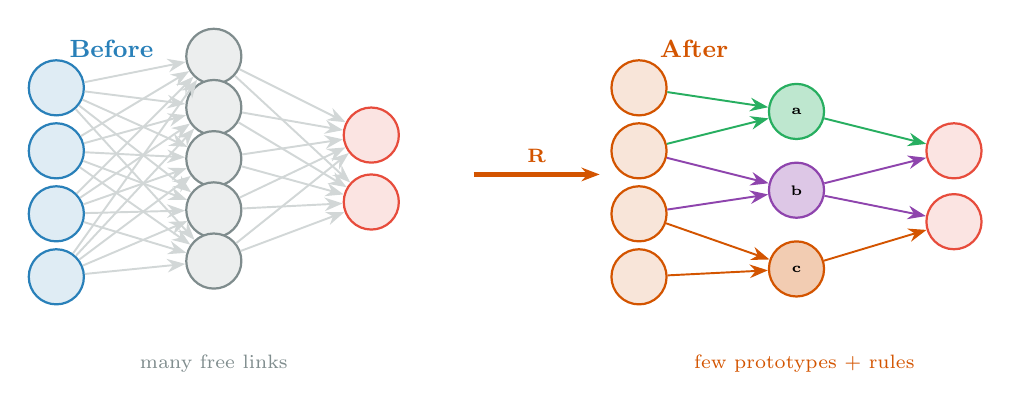
\begin{tikzpicture}[
    >={Stealth[length=2.3mm]},
    neuron/.style={circle, minimum size=7mm, draw, line width=0.8pt, font=\tiny\bfseries},
    arrow/.style={->, thick, line width=0.7pt},
]
\node[font=\small\bfseries, text=teachcol] at (0.7,2.3) {Before};
\foreach \i in {1,...,4} {
    \node[neuron, fill=teachcol!15, draw=teachcol] (inA\i) at (0,{1.8-(\i-1)*0.8}) {};
}
\foreach \j in {1,...,5} {
    \node[neuron, fill=greycol!15, draw=greycol] (hidA\j) at (2,{2.2-(\j-1)*0.65}) {};
}
\foreach \k in {1,...,2} {
    \node[neuron, fill=physcol!15, draw=physcol] (outA\k) at (4,{1.2-(\k-1)*0.85}) {};
}
\foreach \i in {1,...,4} {\foreach \j in {1,...,5} {\draw[arrow, greycol!35] (inA\i) -- (hidA\j);}}
\foreach \j in {1,...,5} {\foreach \k in {1,...,2} {\draw[arrow, greycol!35] (hidA\j) -- (outA\k);}}

\draw[->, ultra thick, structcol, line width=1.8pt] (5.3,0.7) -- node[above, font=\scriptsize\bfseries, text=structcol] {$\mathbf{R}$} (6.9,0.7);

\node[font=\small\bfseries, text=structcol] at (8.1,2.3) {After};
\foreach \i in {1,...,4} {
    \node[neuron, fill=structcol!15, draw=structcol] (inB\i) at (7.4,{1.8-(\i-1)*0.8}) {};
}
\node[neuron, fill=studcol!30, draw=studcol] (h1) at (9.4,1.5) {a};
\node[neuron, fill=clustcol!30, draw=clustcol] (h2) at (9.4,0.5) {b};
\node[neuron, fill=structcol!30, draw=structcol] (h3) at (9.4,-0.5) {c};
\foreach \k in {1,...,2} {
    \node[neuron, fill=physcol!15, draw=physcol] (outB\k) at (11.4,{1.0-(\k-1)*0.9}) {};
}
\draw[arrow, studcol] (inB1) -- (h1);
\draw[arrow, studcol] (inB2) -- (h1);
\draw[arrow, clustcol] (inB2) -- (h2);
\draw[arrow, clustcol] (inB3) -- (h2);
\draw[arrow, structcol] (inB3) -- (h3);
\draw[arrow, structcol] (inB4) -- (h3);
\draw[arrow, studcol] (h1) -- (outB1);
\draw[arrow, clustcol] (h2) -- (outB1);
\draw[arrow, clustcol] (h2) -- (outB2);
\draw[arrow, structcol] (h3) -- (outB2);

\node[font=\scriptsize, text=greycol] at (2,-1.7) {many free links};
\node[font=\scriptsize, text=structcol] at (9.5,-1.7) {few prototypes + rules};
\end{tikzpicture}
\end{center}

The important point is this: the final network is not smaller because we manually deleted neurons. It is smaller because the paper \textbf{proved from the trained weights} that many neurons were redundant.

\section{Results in One Table}

\begin{table}[H]
\centering
\small
\begin{tabularx}{\textwidth}{@{}lCCCC@{}}
\toprule
\textbf{Problem} & \textbf{Standard PINN} & \textbf{PINN-post} & \textbf{$\Psi$-NN} & \textbf{Main Message} \\
\midrule
Laplace & $2.26\times 10^{-2}$ & $7.64\times 10^{-3}$ & $\mathbf{1.03\times 10^{-3}}$ & Finds symmetry and becomes much more accurate \\
Burgers & $2.03\times 10^{-1}$ & $1.14\times 10^{-1}$ & $\mathbf{6.82\times 10^{-2}}$ & Handles anti-symmetry and inverse identification \\
Poisson & $4.20\times 10^{-2}$ & $3.59\times 10^{-2}$ & $\mathbf{1.62\times 10^{-2}}$ & Discovers more complex permutation structure \\
Navier--Stokes & --- & --- & strong transfer & Reuses structures discovered on simpler PDEs \\
\bottomrule
\end{tabularx}
\caption{The paper shows that discovered structure improves both efficiency and accuracy.}
\end{table}

\section{Key Takeaways}

\begin{enumerate}[leftmargin=*]
    \item $\Psi$-NN first solves the physics, then discovers the architecture.
    \item It discovers structure by analyzing trained student weights, not by manual design.
    \item It looks for repeated rows, sign reversals, permutations, and zero links.
    \item It keeps only a few independent prototypes and reconstructs the rest with rules.
    \item The best structure is the smallest one that still preserves physics accuracy.
\end{enumerate}

\section{In One Sentence}

\begin{center}
\fbox{\parbox{0.86\textwidth}{
\centering
$\Psi$-NN automatically discovers structure by compressing a trained physics network into a smaller set of unique weight patterns, then rebuilding a new architecture from those patterns.
}}
\end{center}

\end{document}
